\chapter[Processo de Engenharia de Requisitos]{Processo de Engenharia de Requisitos}
  
  Como foi esclarecido no Capítulo 3, a abordagem a ser utilizada no projeto é uma abordagem híbrida do 
  \textit{Scaled Agile Framework} (SAFe) com o \textit{Rational Unified Process} (RUP).
  
  Para a definição do processo de Engenharia de Requisitos para o projeto, foi mantida a estrutura do SAFe com os seus três níveis,
  o nível de Portfólio, de Programa e de Time (como ilustra a Figura~\ref{safe_big_picture}), e trazidos alguns
  conceitos do RUP, como a utilização de casos de uso a nível de time.
  
  A estrutura dos três níveis do SAFe foi mantida porque, segundo Leffingwell (\citeyear{leffingwell11}),
  ao ir abaixando o nível de abstração dos requisitos mais gradativamente, é reduzido o nível de especificação precoce,
  reduzindo a sobrecarga ao gerenciar os requisitos. Isso também aumenta a agilidade do time por permitir a interpretação
  dos requisitos de maneira mais fácil para a implementação \cite{leffingwell11}.
  
  \begin{figure}[!htbp]
    \centering
    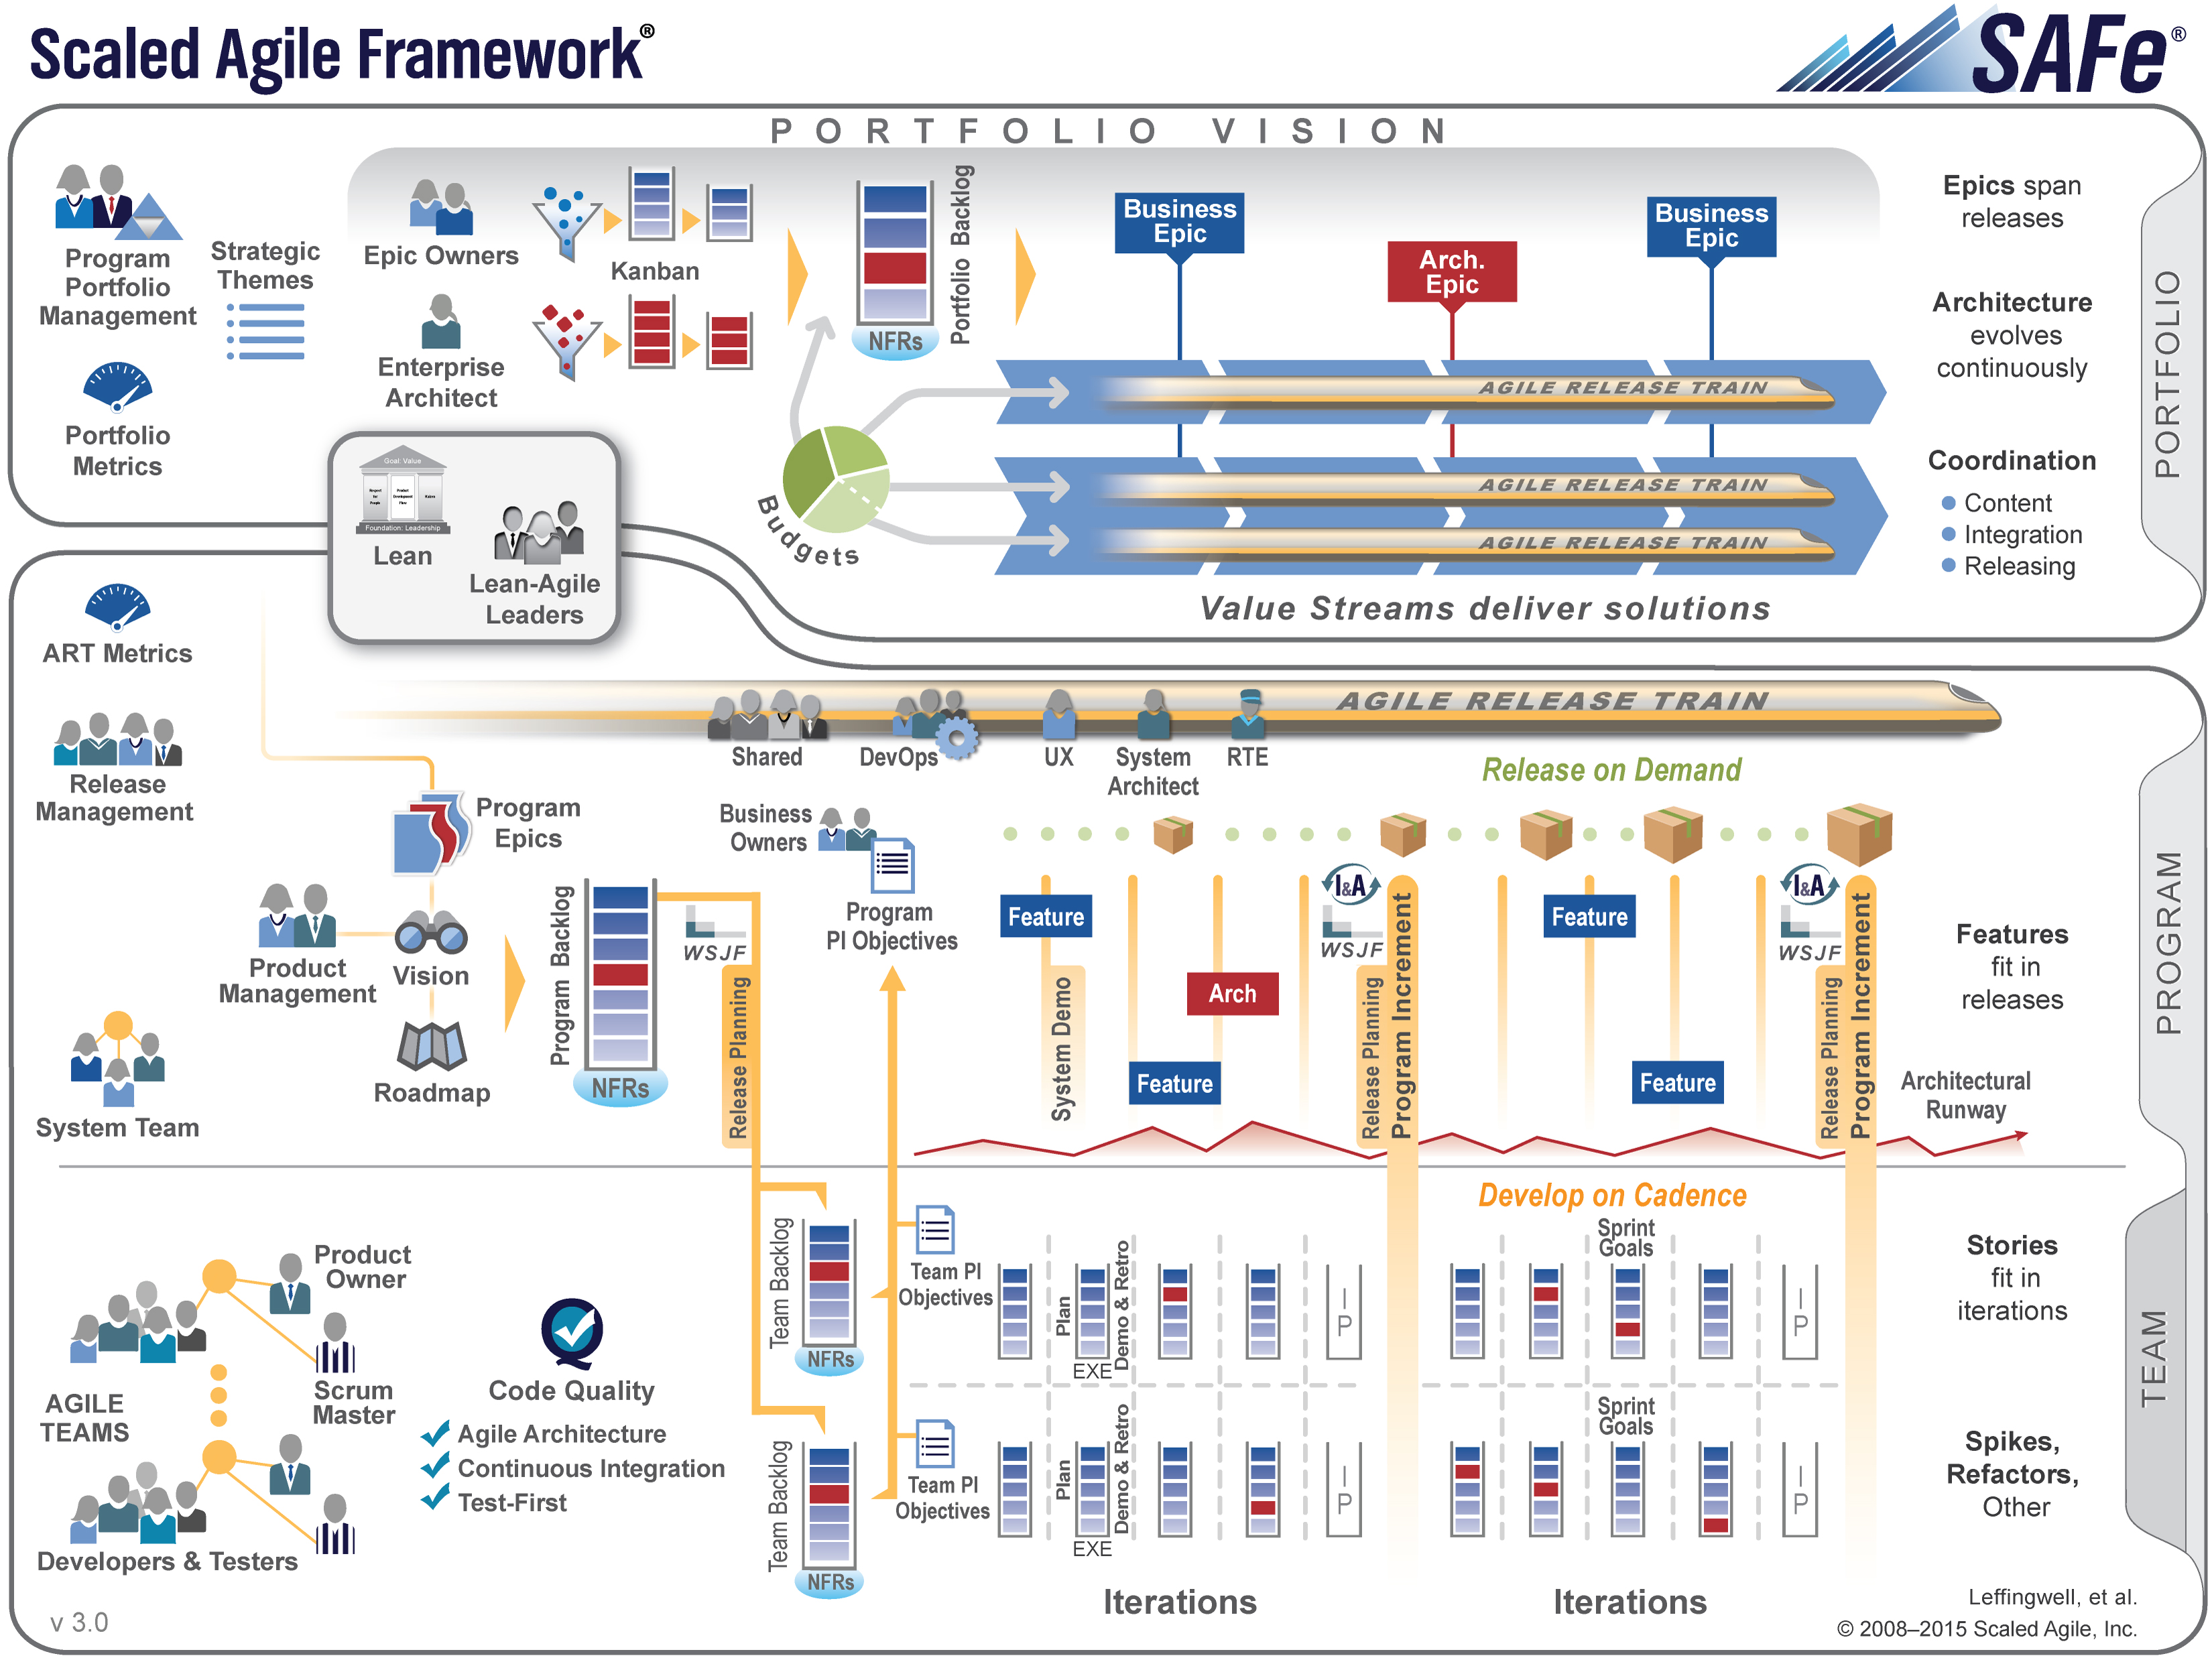
\includegraphics[scale=0.11]{editaveis/figuras/SAFe_Big_Picture}
    \caption[The SAFe Big Picture]{\textit{The Big Picture}: \textit{Framework} proposto pelo SAFe\textregistered. \footnotemark}
    \label{safe_big_picture}
  \end{figure}
  \footnotetext{Fonte: Leffingwell, \textit{et al} (2008-2015). Disponível em <http://www.scaledagileframework.com/>}
  
  As próximas seções tratam sobre o modelo do processo de Engenharia de Requisitos, apelidado de '\textit{Big Picture}
  do projeto', os papéis desempenhados e as atividades e artefatos envolvidos no processo.
  
  \pagebreak
  \section{A '\textit{Big Picture}' do projeto}

        
  \begin{figure}[!htbp]
  \centering
  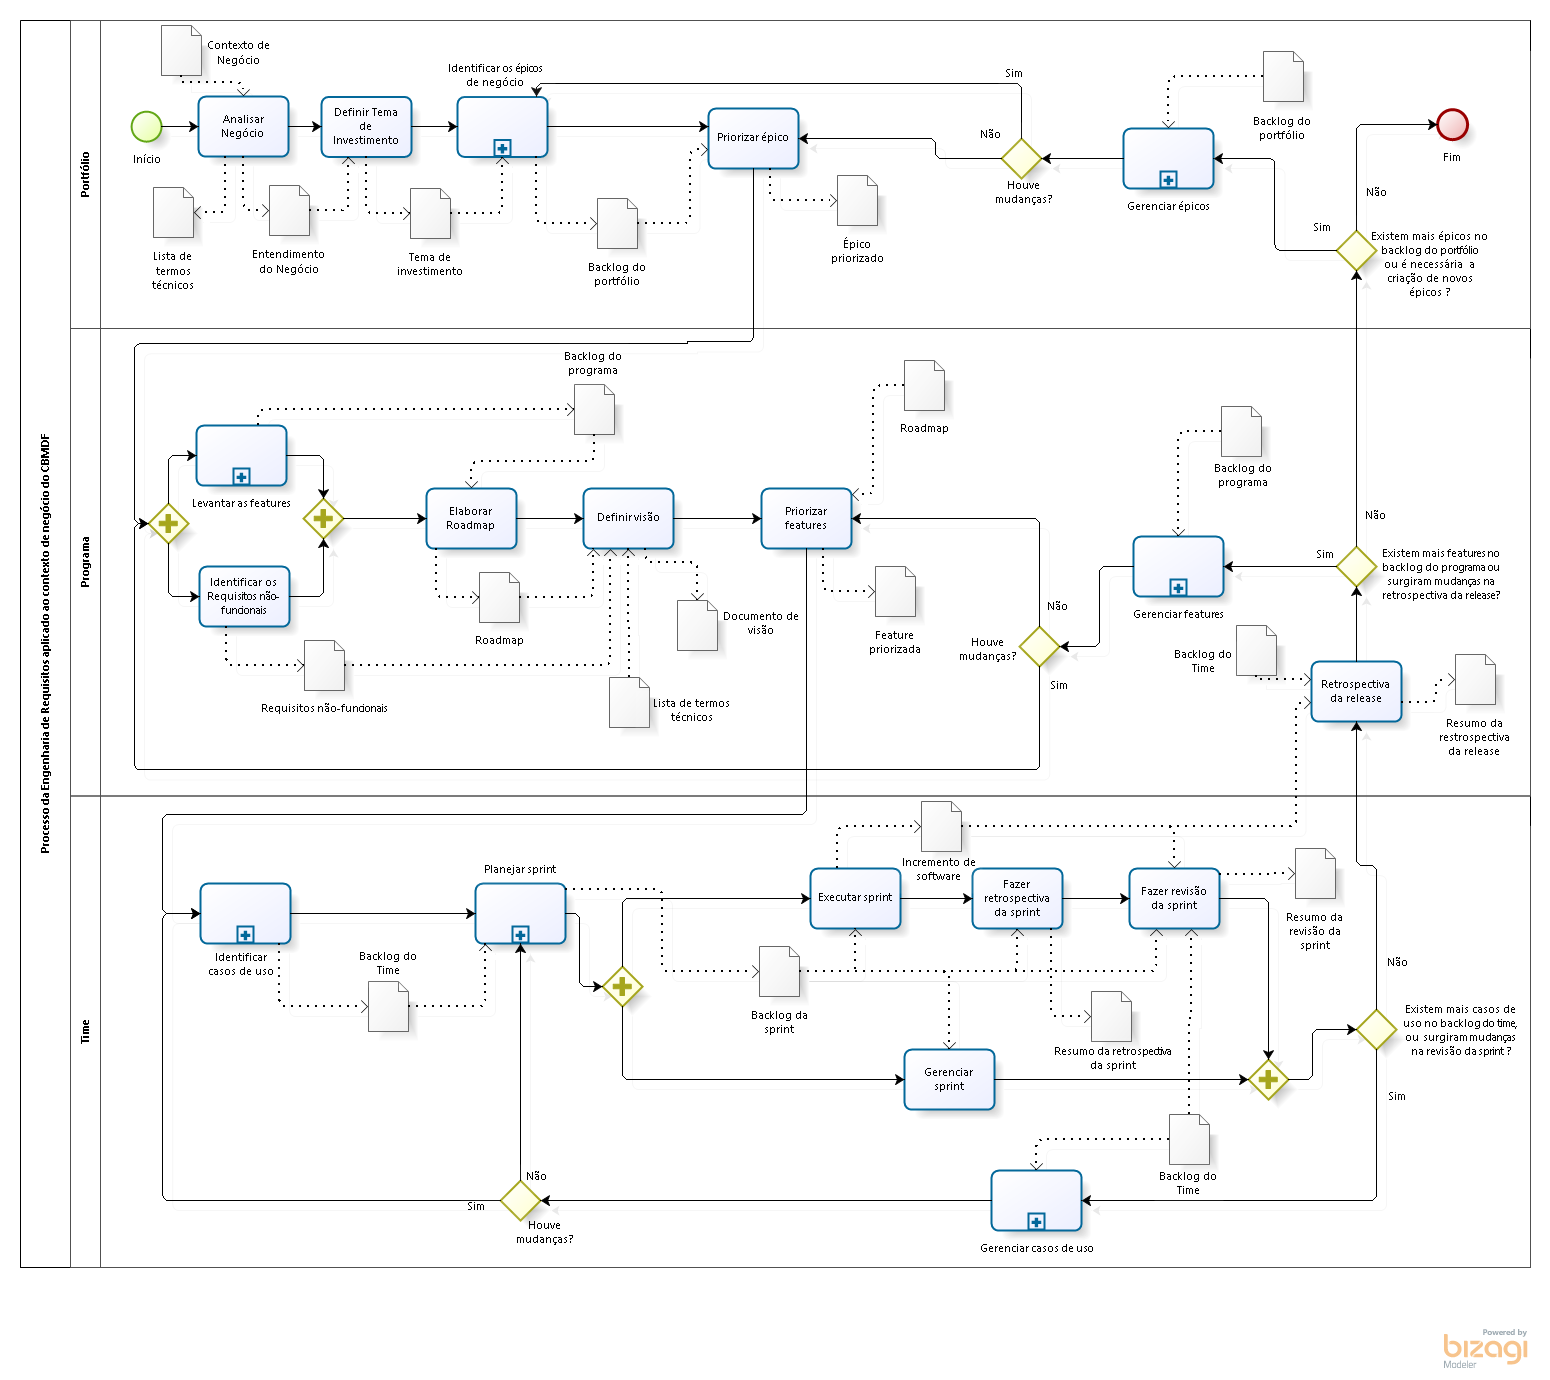
\includegraphics[scale=0.5, angle = 90]{editaveis/figuras/project_big_picture}
  \caption[Modelo do processo de Engenharia de Requisitos: \textit{Big Picture} do projeto]
      {Modelo do processo de Engenharia de Requisitos: \textit{Big Picture} do projeto.}
  \label{project_big_picture}
  \end{figure}
  
  \pagebreak
  \subsection{Subprocessos da '\textit{Big Picture}' do projeto}

    \begin{figure}[!htbp]
      \centering
      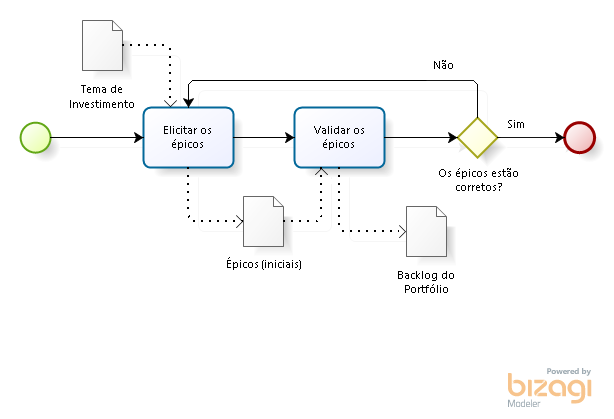
\includegraphics[scale=0.55]{editaveis/figuras/processo_identificar_epicos}
      \caption[Subprocesso - Identificar épicos de negócio]{Subprocesso - Identificar épicos de negócio.}
      \label{processo_identificar_epicos}
    \end{figure}

    \begin{figure}[!htbp]
      \centering
      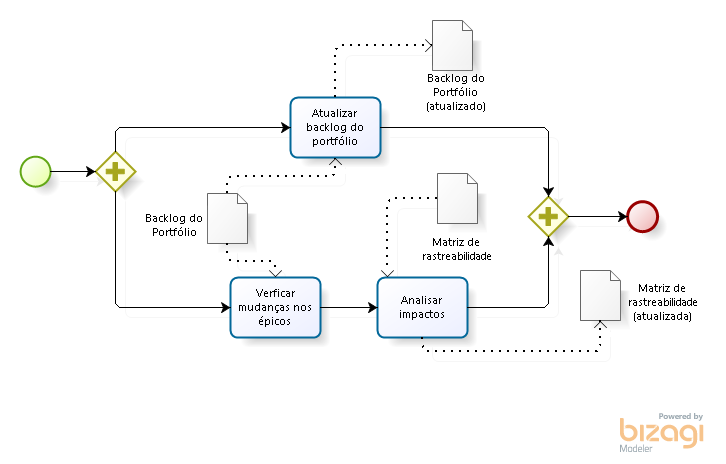
\includegraphics[scale=0.55]{editaveis/figuras/processo_gerenciar_epicos}
      \caption[Subprocesso - Gerenciar épicos]{Subprocesso - Gerenciar épicos.}
      \label{processo_gerenciar_epicos}
    \end{figure}

    \begin{figure}[!htbp]
      \centering
      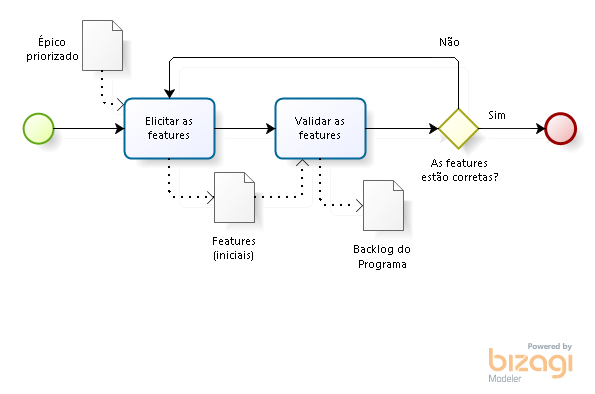
\includegraphics[scale=0.55]{editaveis/figuras/processo_levantar_features}
      \caption[Subprocesso - Levantar \textit{features}]{Subprocesso - Levantar \textit{features}.}
      \label{processo_levantar_features}
    \end{figure}

%     \pagebreak
    \begin{figure}[!htbp]
      \centering
      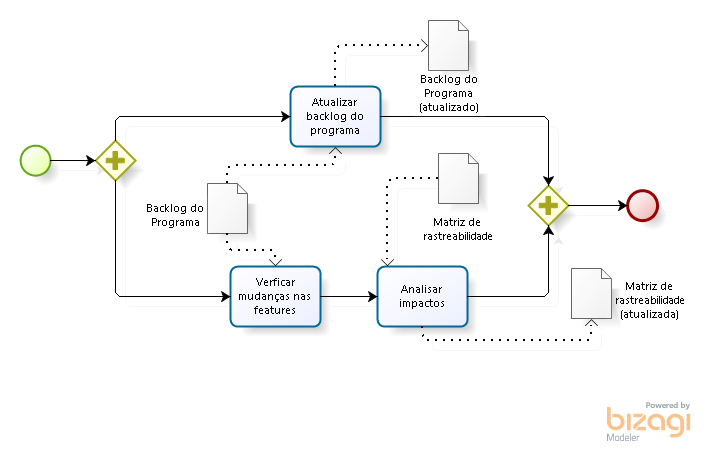
\includegraphics[scale=0.55]{editaveis/figuras/processo_gerenciar_features}
      \caption[Subprocesso - Gerenciar \textit{features}]{Subprocesso - Gerenciar \textit{features}.}
      \label{processo_gerenciar_features}
    \end{figure}

    \begin{figure}[!htbp]
      \centering
      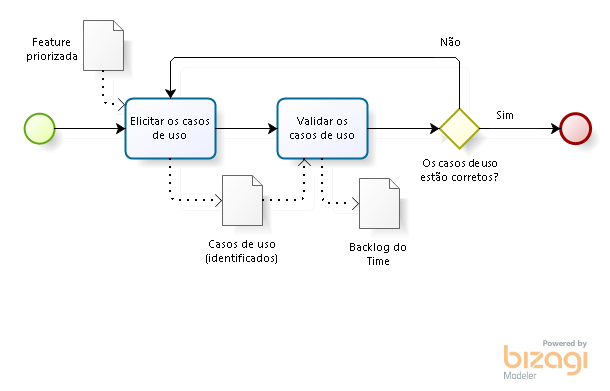
\includegraphics[scale=0.5]{editaveis/figuras/processo_identificar_casos_uso}
      \caption[Subprocesso - Identificar casos de uso]{Subprocesso - Identificar casos de uso.}
      \label{processo_identificar_casos_uso}
    \end{figure}
    
    \begin{figure}[!htbp]
      \centering
      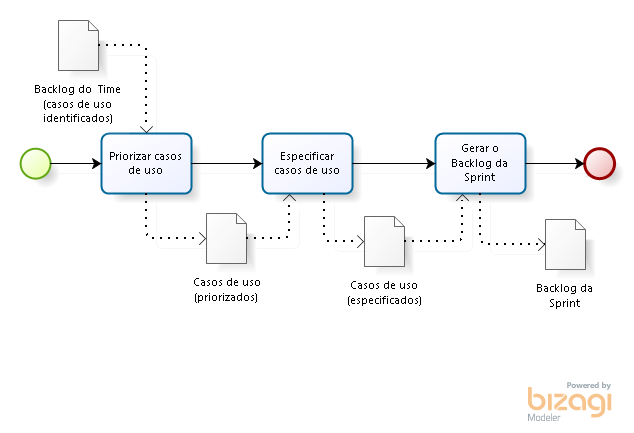
\includegraphics[scale=0.5]{editaveis/figuras/processo_planejar_sprint}
      \caption[Subprocesso - Planejar \textit{Sprint}]{Subprocesso - Planejar \textit{Sprint}.}
      \label{processo_planejar_sprint}
    \end{figure}

    \begin{figure}[!htbp]
      \centering
      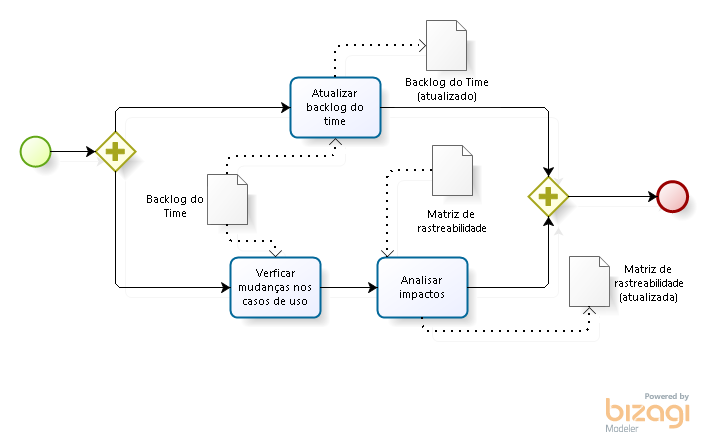
\includegraphics[scale=0.55]{editaveis/figuras/processo_gerenciar_casos_uso}
      \caption[Subprocesso - Gerenciar casos de uso]{Subprocesso - Gerenciar casos de uso.}
      \label{processo_gerenciar_casos_uso}
    \end{figure}
    
  \pagebreak
  \section{Papéis no processo}
    
    
  Os papéis, e responsabilidades dos papéis, definidos para o processo são os seguintes:
  
  \begin{itemize}
   
   \item \textbf{\textit{Especialista do Negócio}}
   
      O Especialista do Negócio é o \textit{stakeholder} que detém o conhecimento do negócio, do contexto organizacional
      e da visão do produto.
      O professor atuará como Especialista do Negócio, majoritariamente, em todos os níveis (Portfólio, Programa e Time).
   
   \item \textbf{\textit{Product Owner} (PO)}
      
      Segundo conceitos apresentados por Leffingwell (\citeyear{leffingwell11}),
      são atividades de responsabilidade do PO, adaptados para o processo do projeto:
      
      \begin{itemize}
       
       \item Trabalhar com o \textit{Product Manager};
       
       \item Definir objetivos para a \textit{sprint};
       
       \item Priorizar e manter o \textit{Backlog} do Time;
       
       \item Elaborar e validar os casos de uso;
       
       \item Participar do planejamento da \textit{sprint} e validar a \textit{sprint}.
       
      \end{itemize}

      
      O professor atuará como PO para fornecer os insumos para as atividades que lhe couber, atuando como Especialista
      do Negócio, como as atividades de validação de \textit{sprints}, validação de casos de uso, entre outras do tipo.
      
      Fica para a equipe de requisitos a responsabilidade da execução das atividades, como planejamento de \textit{sprint},
      manutenção do \textit{Backlog}, entre outras. O papel do PO será exercido por membros da equipe de requisitos.
      
      O PO atuará no nível de Time.
      
   \item \textbf{\textit{Product Manager} (PM)}
      
      Segundo conceitos apresentados por Leffingwell (\citeyear{leffingwell11}),
      são atividades de responsabilidade do PM, adaptados para o processo do projeto:
      
      \begin{itemize}
       
       \item Manter a Visão e o \textit{Backlog do Programa};
       
       \item Priorizar \textit{features} e manter o \textit{Roadmap};
       
       \item Gerenciar o conteúdo da \textit{release};
       
       \item Manter e priorizar o \textit{Backlog do Portfólio};
       
      \end{itemize}
      
      O papel do PM será exercido por membros da equipe de requisitos, onde o professor atuará como Especialista de Negócio para
      o fornecimento das informações necessárias.
      
      O PM atuará nos níveis de programa e portfólio, atuando nas atividades relacionadas
      aos requisitos de mais alto nível.
      
      
   \item \textbf{\textit{Scrum Master}}
      
      O \textit{Scrum Master} é responsável por assistir o time para garantir a melhor perfomance, atuando com 
      um líder do time \cite{leffingwell11}.
      São responsabilidades do \textit{Scrum Master}, segundo Leffingwell (\citeyear{leffingwell11}):
      
      \begin{itemize}
       
       \item Facilitar o progresso do time;
       
       \item Liderar os esforços do time;
       
       \item Eliminar impedimentos;
       
      \end{itemize}
      
      O papel do \textit{Scrum Master} será realizado por um integrante da equipe de requisitos.
      
   \item \textbf{Time}
      
      O time é composto pelos desenvolvedores, que é representado por toda a equipe de requisitos.	
      
  \end{itemize}
  
  \vfill
    
  \pagebreak
  \section{Atividades e artefatos do processo}
    
    Nesta seção são abordadas os conceitos dos artefatos envolvidos no processo, bem como as atividades que se relacionam com
    esses artefatos.
    
      
  \subsection{Artefatos envolvidos}
  
    São listados abaixo os conceitos de alguns artefatos utilizados no processo, no contexto do projeto,
    para o melhor entendimento das atividades do processo.
    
    \begin{itemize}
     
     \item \textbf{Temas de Investimento} - Representa o conjunto de iniciativas que coordenam o portfólio da organização \cite{leffingwell11}.
      Os épicos são derivados a partir de um Tema de Investimento.
     
     \item \textbf{Épicos} - São iniciativas de desenvolvimento em larga escala que agregam valor a um tema de investimento \cite{leffingwell11}.
     São os artefatos de requisitos de mais alto nível no processo \cite{leffingwell11}.
     São decompostos em \textit{features}.
     
     \item \textbf{\textit{Backlog} do Portfólio} - É o repositório dos épicos.
     
     \item \textbf{\textit{Features}} - São serviços fornecidos pelo sistema que atendem às necessidades dos
     \textit{stakeholders} \cite{leffingwell03}. As \textit{features} atuam como pontes entre as necessidades
     dos \textit{stakeholders} (requisitos de alto nível) e os requisitos específicos no domínio da solução \cite{leffingwell11}.
     São decompostas em casos de uso.
     
     \item \textbf{Requisitos não-funcionais} - São qualidades do sistema, que caracterizam o comportamento do mesmo.
      Serão armazenados no Documento de Visão do projeto e serão escritos baseado no modelo de Especificações Suplementares
      fornecido por Leffingwell e Widrig (\citeyear{leffingwell03}).
     
     \item \textbf{\textit{Backlog} do Programa} - É o repositório das \textit{features} do sistema.
     
     \item \textbf{\textit{Roadmap}} - Consiste em um conjunto de \textit{releases} com datas planejadas, cada uma com um tema,
     um conjunto de \textit{features} priorizadas e um conjunto de objetivos, demonstrando a intenção da empresa em mostrar valor ao
     longo do tempo \cite{leffingwell11}.
     
     \item \textbf{Documento de Visão} - É um mecanismo para definir e comunicar a Visão do sistema \cite{leffingwell11}.
      O conteúdo primário da Visão de um sistema é o conjunto de \textit{features} priorizadas que descrevem o que o sistema
      será capaz de oferecer a seus usuários, para atender as necessidades dos envolvidos \cite{leffingwell11}.
      O Documento de Visão do projeto armazenará também os requisitos não-funcionais e os termos técnicos identificados na
      análise do negócio, entre outras informações importantes.
 
     \item \textbf{Casos de Uso} - Um caso de uso captura um contrato sobre o comportamento de um sistema
      entre os \textit{stakeholders} desse sistema \cite{cockburn01}.
      Descreve o comportamento do sistema frente a várias condições, enquanto o sistema responde a
      um pedido de um dos \textit{stakeholders} \cite{cockburn01}. Os casos de uso fornecem parte do insumo para a implementação.
      
     \item \textbf{\textit{Backlog} do Time} - É o repositório dos casos de uso que serão desenvolvidos em uma \textit{release}.
     
     \item \textbf{\textit{Backlog} da Sprint} - É o repositório dos casos de uso que serão desenvolvidos em uma \textit{sprint}.
     
     \item \textbf{Incremento de \textit{software}} - É a porção do \textit{software} que é gerado em cada \textit{sprint}.
     
     \item \textbf{\textit{Build}} - É o conjunto dos incrementos de \textit{software} que foram gerados em cada \textit{sprint}
      durante uma \textit{release}.
     
    \end{itemize}

  \subsection{Atividades e seus artefatos}
    
    A seguir são descritas as atividades e os artefatos envolvidos no processo em cada nível do SAFe, Portfólio, Programa e Time.
    
    
  \subsubsection{Nível de Portfólio}
    
    \begin{itemize}
      
      \item Atividade \textbf{Analisar o negócio}
	  
	  \begin{itemize}
	    \item \textbf{Artefato(s) de entrada}: Contexto de negócio, Processo atual de negócio.
	    
	    \item \textbf{Descrição}: Esta atividade tem por objetivo entender o contexto do negócio, os problemas de mais alto nível
	      e estabelecer um vocabulário comum entre a equipe de desenvolvimento e o cliente, validando os resultados com os
	      \textit{stakeholders}.
	    
	    \item \textbf{Artefato(s) de saída}: Lista de termos técnicos, Entendimento do Negócio.
	      
	  \end{itemize}
     
     \item Atividade \textbf{Definir Tema de Investimento}
	
	\begin{itemize}
	  \item \textbf{Artefato(s) de entrada}: Entendimento do Negócio.
	  
	  \item \textbf{Descrição}: Esta atividade consiste em definir o Tema de Investimento da organização,
	    para a derivação dos épicos.
	  
	  \item \textbf{Artefato(s) de saída}: Tema de Investimento definido.
	 	 
	\end{itemize}
	
     \item Subprocesso \textbf{Identificar os épicos de negócio}
	
	\begin{itemize}
	  
	  \item Atividade \textbf{Elicitar os épicos}
	  
	      \begin{itemize}
		\item \textbf{Artefato(s) de entrada}: Tema de Investimento.
		
		\item \textbf{Descrição}: Esta atividade tem por objetivo abstrair do Tema de Investimento definido as
		  iniciativas de desenvolvimento em larga escala (épicos), juntamente com os \textit{stakeholders},
		  a partir das técnicas de elicitação definidas.
		
		\item \textbf{Artefato(s) de saída}: Épicos (iniciais).
		      
	      \end{itemize}
	      
	  \item Atividade \textbf{Validar os épicos}
	  
	      \begin{itemize}
		\item \textbf{Artefato(s) de entrada}: Épicos (iniciais).
		
		\item \textbf{Descrição}: Esta atividade tem por objetivo validar os épicos que foram elicitados, juntamente
		com os \textit{stakeholders}. O \textit{Backlog} do Portfólio será composto dos épicos validados pelos
		\textit{stakeholders}.
		
		\item \textbf{Artefato(s) de saída}: \textit{Backlog} do Portfólio.
		      
	      \end{itemize}
	\end{itemize} % Fim das atividades de um subprocesso
	      
      \item Atividade \textbf{Priorizar épico}
      
	  \begin{itemize}
	    \item \textbf{Artefato(s) de entrada}: \textit{Backlog}  do Portfólio.
	    
	    \item \textbf{Descrição}: Esta atividade tem por objetivo definir o épico de maior relevância de onde serão
	      abstraídas as \textit{features}.
	    
	    \item \textbf{Artefato(s) de saída}: Épico priorizado.
		  
	  \end{itemize}
	   
	
     \item Subprocesso \textbf{Gerenciar épicos}
     
	\begin{itemize}
	 
	 \item Atividade \textbf{Atualizar \textit{Backlog} do Portfólio}
	    
	    \begin{itemize}
	      \item \textbf{Artefato(s) de entrada}: \textit{Backlog} do Portfólio.

	      \item \textbf{Descrição}: Consiste no acompanhamento do \textit{Backlog} do Portfólio, atualizando eventuais
		mudanças e épicos que já foram implementados e revisados.
	      
	      \item \textbf{Artefato(s) de saída}: \textit{Backlog} do Portfólio (atualizado).
		    
	    \end{itemize}
	    
	 \item Atividade \textbf{Verificar mudanças nos épicos}
	    
	    \begin{itemize}
	      \item \textbf{Artefato(s) de entrada}: \textit{Backlog} do Portfólio.

	      \item \textbf{Descrição}: Consiste em verificar se são necessárias mudanças nos épicos do
		\textit{Backlog} do Portfólio.
	      
	      \item \textbf{Artefato(s) de saída}: \textit{Backlog} do Portfólio (atualizado), se houver mudanças.
		    
	    \end{itemize}
	    
	 \item Atividade \textbf{Analisar impactos}
	    
	    \begin{itemize}
	      \item \textbf{Artefato(s) de entrada}: Matriz de rastreabilidade.

	      \item \textbf{Descrição}: Consiste em analisar os impactos causados por uma mudança em um ou
		mais épicos, e mitigar o problema, se houver.
	      
	      \item \textbf{Artefato(s) de saída}: Matriz de rastreabilidade (atualizada).
		    
	    \end{itemize}
	    
	\end{itemize}
     
    \end{itemize}
    
    \vfill
    
    \pagebreak
    
  \subsubsection{Nível de Programa}
    
    \begin{itemize}
	
     \item Subprocesso \textbf{Levantar as \textit{features}}
	
	\begin{itemize}
	  \item Atividade \textbf{Elicitar as \textit{features}}
	      
	      \begin{itemize}
		  \item \textbf{Artefato(s) de entrada}: Épico priorizado.
		  
		  \item \textbf{Descrição}: Esta atividade tem por objetivo abstrair do épico priorizado
		    as \textit{features} necessárias, juntamente com os \textit{stakeholders}, a partir das
		    técnicas de elicitação definidas.
		  
		  \item \textbf{Artefato(s) de saída}: \textit{Features} (iniciais).
		    
		\end{itemize}
	    
	    \item Atividade \textbf{Validar as \textit{features}}
	    
		\begin{itemize}
		  \item \textbf{Artefato(s) de entrada}: \textit{Features} (iniciais).
		  
		  \item \textbf{Descrição}: Esta atividade consiste em validar as \textit{features} elicitadas,
		    juntamente com os \textit{stakeholders}. O \textit{Backlog} do Programa será composto
		    pelas \textit{features} validadas pelos \textit{stakeholders}.
		  
		  \item \textbf{Artefato(s) de saída}: \textit{Backlog} do Programa.
			
		\end{itemize}
	\end{itemize} % Fim das atividades de um subprocesso
	      
     \item Atividade \textbf{Identificar os Requisitos não-funcionais}
      
	  \begin{itemize}
	    \item \textbf{Artefato(s) de entrada}: Nenhum.
	    
	    \item \textbf{Descrição}: Esta atividade tem por objetivo abstrair das necessidades do cliente os
	      requisitos não-funcionais do sistema. Se já houver requisitos não-funcionais identificados para o sistema,
	      os mesmos deverão ser consultados para atualizações.
	    
	    \item \textbf{Artefato(s) de saída}: Requisitos não-funcionais.
		  
	  \end{itemize}
	  
     \item Atividade \textbf{Elaborar \textit{Roadmap}}
      
	  \begin{itemize}
	    \item \textbf{Artefato(s) de entrada}: \textit{Backlog} do Programa.
	    
	    \item \textbf{Descrição}: Esta atividade tem por objetivo priorizar as \textit{features} do
	      \textit{Backlog} do Programa, planejando o arranjo das mesmas nas \textit{releases}.  Caso já exista
	      um \textit{Roadmap}, o mesmo deve ser atualizado com eventuais mudanças.
	    
	    \item \textbf{Artefato(s) de saída}: \textit{Roadmap}.
		  
	  \end{itemize}
	  
     \item Atividade \textbf{Definir Visão}
      
	  \begin{itemize}
	    \item \textbf{Artefato(s) de entrada}: Lista de termos técnicos, Requisitos não-funcionais e \textit{Roadmap}.
	    
	    \item \textbf{Descrição}: Esta atividade tem por objetivo elaborar (ou atualizar, caso já exista um
	      documento de visão) o documento de visão.
	    
	    \item \textbf{Artefato(s) de saída}: Documento de Visão.
		  
	  \end{itemize}
	  
     \item Atividade \textbf{Priorizar uma \textit{feature}}
      
	  \begin{itemize}
	    \item \textbf{Artefato(s) de entrada}: \textit{Roadmap}.
	    
	    \item \textbf{Descrição}: Esta atividade consiste em definir a \textit{feature} de maior relevância
	      de onde serão derivados os casos de uso.
	    
	    \item \textbf{Artefato(s) de saída}: \textit{Feature} priorizada.
		  
	  \end{itemize}
	
     \item Subprocesso \textbf{Gerenciar \textit{features}}
     
	\begin{itemize}
	 
	 \item Atividade \textbf{Atualizar \textit{Backlog} do Programa}
	    
	    \begin{itemize}
	      \item \textbf{Artefato(s) de entrada}: \textit{Backlog} do Programa.

	      \item \textbf{Descrição}: Consiste no acompanhamento do \textit{Backlog} do Programa, atualizando
		eventuais mudanças e \textit{features} que já foram implementadas e revisadas.
	      
	      \item \textbf{Artefato(s) de saída}: \textit{Backlog} do Programa (atualizado).
		    
	    \end{itemize}
	    
	 \item Atividade \textbf{Verificar mudanças nas \textit{features}}
	    
	    \begin{itemize}
	      \item \textbf{Artefato(s) de entrada}: \textit{Backlog} do Programa.

	      \item \textbf{Descrição}: Consiste em verificar se são necessárias mudanças nas \textit{features} do
		\textit{Backlog} do Programa.
	      
	      \item \textbf{Artefato(s) de saída}: \textit{Backlog} do Programa (atualizado), se houver mudanças.
		    
	    \end{itemize}
	    
	 \item Atividade \textbf{Analisar impactos}
	    
	    \begin{itemize}
	      \item \textbf{Artefato(s) de entrada}: Matriz de rastreabilidade.

	      \item \textbf{Descrição}: Consiste em analisar os impactos causados por uma mudança em uma ou mais
		\textit{features}, e mitigar o problema, se houver.
	      
	      \item \textbf{Artefato(s) de saída}: Matriz de rastreabilidade (atualizada).
		    
	    \end{itemize}
	    
	\end{itemize}
	
     \item Atividade \textbf{Restrospectiva da \textit{release}}
      
	  \begin{itemize}
	    \item \textbf{Artefato(s) de entrada}: \textit{Backlog} do Time e
	      Incremento de \textit{software} (\textit{Build} produzida pelo time na \textit{release}).
	    
	    \item \textbf{Descrição}: Esta atividade tem por objetivo validar o que foi produzido na \textit{release},
	      juntamente com os envolvidos.
	    
	    \item \textbf{Artefato(s) de saída}: Resumo da retrospectiva da \textit{release}.
		  
	  \end{itemize}
     
    \end{itemize}
    
    \pagebreak
    
  \subsubsection{Nível de Time}
    
    \begin{itemize}
	
     \item Subprocesso \textbf{Especificar Casos de Uso}
	
	\begin{itemize}
	  \item Atividade \textbf{Elicitar casos de uso}
	      
	      \begin{itemize}
		  \item \textbf{Artefato(s) de entrada}: \textit{Feature} priorizada.
		  
		  \item \textbf{Descrição}: Consiste em levantar os casos de uso juntamente com os clientes
		    (\textit{stakeholders}), utilizando as técnicas de elicitação definidas,  a partir de determinada
		    \textit{feature}.
		  
		  \item \textbf{Artefato(s) de saída}: Casos de uso (iniciais).
		    
		\end{itemize}
	    
	    \item Atividade \textbf{Validar casos de uso}.
	    
		\begin{itemize}
		  \item \textbf{Artefato(s) de entrada}: Casos de uso (iniciais).
		  
		  \item \textbf{Descrição}: Consiste em validar os casos de uso elicitados, juntamente com os
		    clientes (\textit{stakeholders}).
		  
		  \item \textbf{Artefato(s) de saída}: \textit{Backlog} do Time com os casos de uso que foram validados.
			
		\end{itemize}
		
	    \item Atividade \textbf{Escrever a descrição dos casos de uso}.
	    
		\begin{itemize}
		  \item \textbf{Artefato(s) de entrada}: \textit{Backlog} do Time.
		  
		  \item \textbf{Descrição}: Consiste em descrever detalhadamente os casos de uso do \textit{Backlog} do time.
		  
		  \item \textbf{Artefato(s) de saída}: Descrição dos casos de uso.
			
		\end{itemize}
		
	    \item Atividade \textbf{Elaborar diagrama de casos de uso}.
	    
		\begin{itemize}
		  \item \textbf{Artefato(s) de entrada}: Casos de uso (iniciais).
		  
		  \item \textbf{Descrição}: Consiste em modelar (UML) os casos de uso do \textit{Backlog} do time.
		  
		  \item \textbf{Artefato(s) de saída}: Diagrama de casos de uso.
			
		\end{itemize}
		
	    \item Atividade \textbf{Elaborar modelos de casos de uso}.
	    
		\begin{itemize}
		  \item \textbf{Artefato(s) de entrada}: Descrição de casos de uso e Diagrama de casos de uso.
		  
		  \item \textbf{Descrição}: Consiste em construir o modelo de casos de uso, juntando a descrição dos
		    casos de uso e o diagrama de casos de uso.
		  
		  \item \textbf{Artefato(s) de saída}: Modelos de casos de uso.
			
		\end{itemize}
	\end{itemize} % Fim das atividades de um subprocesso
	      
     \item Atividade \textbf{Priorizar casos de uso}.
      
	  \begin{itemize}
	    \item \textbf{Artefato(s) de entrada}: \textit{Backlog} do Time.
	    
	    \item \textbf{Descrição}: Consiste em priorizar os casos de uso do \textit{Backlog} do Time para
	      encaixá-los em uma \textit{release} (conjunto de \textit{sprints}).
	    
	    \item \textbf{Artefato(s) de saída}: \textit{Backlog} do Time (priorizado).
		  
	  \end{itemize}
	  
     \item Atividade \textbf{Planejar \textit{sprint}}
      
	  \begin{itemize}
	    \item \textbf{Artefato(s) de entrada}: \textit{Backlog} do Programa.
	    
	    \item \textbf{Descrição}: Consiste em selecionar os casos de uso do \textit{Backlog} do time que serão
	      implementados na \textit{sprint}, criando o \textit{Backlog} da \textit{sprint}, e dividir as
	      responsabilidades de desenvolvimento para os integrantes do time.
	    
	    \item \textbf{Artefato(s) de saída}: \textit{Backlog} da \textit{sprint}.
		  
	  \end{itemize}
	  
     \item Atividade \textbf{Executar \textit{sprint}}
      
	  \begin{itemize}
	    \item \textbf{Artefato(s) de entrada}: \textit{Backlog} da \textit{sprint}.
	    
	    \item \textbf{Descrição}: Consiste em implementar os casos de uso do \textit{Backlog} da \textit{sprint}
	      e validar o que foi feito a cada término com o time, além das reuniões diárias (\textit{stand-up meeting}).
	    
	    \item \textbf{Artefato(s) de saída}: Incremento de \textit{software} (\textit{Build}).
		  
	  \end{itemize}
	  
     \item Atividade \textbf{Fazer restrospectiva da \textit{sprint}}
      
	  \begin{itemize}
	    \item \textbf{Artefato(s) de entrada}: \textit{Backlog} da \textit{sprint}.
	    
	    \item \textbf{Descrição}: Consiste numa reunião do time para avaliar o que foi feito e analisar pontos
	      positivos, pontos negativos e possíveis melhorias para a próxima \textit{sprint}.
	    
	    \item \textbf{Artefato(s) de saída}: Resumo da retrospectiva, com os pontos levantados pela equipe
	     (possível \textit{KanBan} de retrospectiva).
		  
	  \end{itemize}
	  
     \item Atividade \textbf{Fazer revisão da \textit{sprint}}
      
	  \begin{itemize}
	    \item \textbf{Artefato(s) de entrada}: \textit{Backlog} da \textit{sprint}, \textit{Backlog} do time,
	      Incremento de \textit{software} gerado na \textit{sprint} (\textit{Build}).
	    
	    \item \textbf{Descrição}: Consiste numa reunião com os envolvidos para avaliar o que foi gerado na \textit{sprint}.
	      Permite alinhar a visão do time com a dos \textit{stakeholders}, verificando se o que foi feito está
	      alinhado com os propósitos iniciais e se haverá mudanças no que será feita em seguida (\textit{Backlog} do time).
	      	    
	    \item \textbf{Artefato(s) de saída}: Resumo da revisão da \textit{sprint}.
		  
	  \end{itemize}
	  
      \item Atividade \textbf{Gerenciar a \textit{sprint}}
      
	  \begin{itemize}
	    \item \textbf{Artefato(s) de entrada}: \textit{Backlog} da \textit{sprint}.
	    
	    \item \textbf{Descrição}: Consiste no acompanhamento e suporte do time durante a \textit{sprint},
	      gerindo o desenvolvimento e possíveis mudanças.
	    
	    \item \textbf{Artefato(s) de saída}: Nenhum.
		  
	  \end{itemize}
	
     \item Subprocesso \textbf{Gerenciar casos de uso}
     
	\begin{itemize}
	 
	 \item Atividade \textbf{Atualizar \textit{Backlog} do Time}
	    
	    \begin{itemize}
	      \item \textbf{Artefato(s) de entrada}: \textit{Backlog} do Time.

	      \item \textbf{Descrição}: Consiste no acompanhamento do \textit{Backlog} do Time, atualizando eventuais
		mudanças e casos de uso que já foram implementados e revisados.
	      
	      \item \textbf{Artefato(s) de saída}: \textit{Backlog} do Time (atualizado).
		    
	    \end{itemize}
	    
	 \item Atividade \textbf{Verificar mudanças nos casos de uso}
	    
	    \begin{itemize}
	      \item \textbf{Artefato(s) de entrada}: \textit{Backlog} do Time e Resumo da revisão de \textit{sprint}.

	      \item \textbf{Descrição}: Consiste em verificar se são necessárias mudanças nos casos de uso do \textit{Backlog}
		do Time. Pode acontecer mudanças dependendo do resultado da revisão de \textit{sprint}.
	      
	      \item \textbf{Artefato(s) de saída}: \textit{Backlog} do Time (atualizado).
		    
	    \end{itemize}
	    
	 \item Atividade \textbf{Analisar impactos}
	    
	    \begin{itemize}
	      \item \textbf{Artefato(s) de entrada}: Matriz de rastreabilidade.

	      \item \textbf{Descrição}: Consiste em analisar os impactos causados por uma mudança em um ou mais casos de uso
	       em outros casos de uso, e mitigar o problema, se houver.
	      
	      \item \textbf{Artefato(s) de saída}: Matriz de rastreabilidade (atualizada).
		    
	    \end{itemize}
	    
	\end{itemize}
	     
    \end{itemize}

    
    
  
  \pagebreak
  \section{Relação com o modelo de maturidade}
  
          
   \subsection{O Modelo de Maturidade MPS.BR}
        
      O modelo de maturidade escolhido para se buscar os processos foi o Melhoria de Processo do \textit{Software} Brasileiro (MPS.BR).
      
      O MPS.BR é um programa mobilizador que visa a melhoria do processo de \textit{software} e serviços, focado principalmente
      para as micro, pequenas e médias empresas \cite{softex12}.
      Uma das bases técnicas para a definição do modelo MPS é o \textit{Capability Maturity Model Integration} (CMMI), mais especificamente
      o \textit{CMMI for Development} (CMMI-DEV\textregistered), sendo compatível com este \cite{softex12}.
      
      O modelo MPS possui quatro componentes, o Modelo de Referência MPS para \textit{Software} (MR-MPS-SW), Modelo de Referência MPS para
      Serviços (MR-MPS-SV), Método de Avaliação (MA-MPS) e Modelo de Negócio (MN-MPS), onde cada componente é descrito por um guia
      do programa MPS.BR \cite{softex12}.
      O guia utilizado para a projeto foi o do MR-MPS-SW, que traz a descrição do Modelo de Referência MPS para \textit{Software}.
      
      O MR-MPS-SW é estruturado em sete níveis de maturidade (de A a G), onde cada nível possui seus respectivos processos \cite{softex12}.
      Os processos do MR-MPS-SW são descritos por meio de propósito e resultados esperados \cite{softex12}.
      Apenas dois níveis de maturidade, o G e o D, contém atividades da Engenharia de Requisitos.
      
    \subsection{Processos e Resultados Esperados do MPS.BR atendidos pelo processo}
    
      O guia não traz as atividades e tarefas necessárias para o atendimento dos propósitos e dos resultados esperados, portanto,
      utilizamos a abordagem e o processo definidos para buscar tais atividades de modo a cumprir os seguintes processos
      e seus resultados esperados:\linebreak
      
      \noindent
      \textbf{Nível G} - Processo \textbf{Gerenciamento de Requisitos (GRE)}
	  
	  \noindent
	  Resultados esperados:
	  
	  \begin{itemize}
	    
	    \item \textbf{GRE 1}: O entendimento dos requisitos é obtido junto aos fornecedores de requisitos;
	      
	      Esse resultado é obtido com as atividades dos subprocessos "Identificar os épicos de negócio", "Levantar as features" 
	      e "Especificar casos de uso", assim como nas atividades "Fazer revisão da \textit{sprint}" 
	      e "Fazer retrospectiva da \textit{release}", onde a participação dos \textit{stakeholders} é marcante para
	      o entendimento dos requisitos.
		  
	    \item \textbf{GRE 3}: A rastreabilidade bidirecional entre os requisitos e os produtos de trabalho é estabelecida e mantida;
	      
	      Esse resultado é obtido com a rastreabilidade que é feita a partir dos artefatos de requisitos do processo,
	      onde um Tema de Investimento gera vários épicos, os épicos geram várias \textit{features} e 
	      as \textit{features} geram vários casos de uso. É possível fazer também o caminho inverso,
	      identificar a partir de um caso de uso, sua respectiva \textit{feature}, dessa \textit{feature} seu respectivo épico, e 
	      deste épico seu respectivo Tema de Investimento.
	    
	    \item \textbf{GRE 4}: Revisões em planos e produtos de trabalho do projeto são realizadas visando identificar
	      e corrigir inconsistências em relação aos requisitos;
	    
	      Esse resultado é obtido com as atividades de "Fazer revisão da \textit{sprint}" 
	      e "Fazer retrospectiva da \textit{release}", onde são validados os requisitos implementados para assegurar
	      a conformidade com os propósitos iniciais do projeto. Além da validação que é feita em diversos documentos,
	      como o Documento de Visão.
	    
	    \item \textbf{GRE 5}: Mudanças nos requisitos são gerenciadas ao longo do projeto.
	    
	      Esse resultado é obtido com as atividades dos subprocessos "Gerenciar Épicos", "Gerenciar \textit{Features}"  e
	      "Gerenciar casos de uso", e a atividade "Gerenciar \textit{sprint}", que tratam das mudanças que podem ocorrer
	      nos requisitos ao longo do projeto.
	      
	  \end{itemize}

      \noindent
      \textbf{Nível D} - Processo \textbf{Desenvolvimento de Requisitos (DRE)}
	  
	  \noindent
	  Resultados esperados:
	  
	  \begin{itemize}
	  
	  \item \textbf{DRE 1}: As necessidades, expectativas e restrições do cliente, tanto do produto quanto
	    de suas interfaces, são identificadas;
	    
	    Esse resultado é obtido através da atividade "Analisar o Negócio" do subprocesso "Identificar os épicos de negócio",
	    ao se levantar as necessidades do cliente frente ao contexto organizacional.
	  
	  \item \textbf{DRE 2}: Um conjunto definido de requisitos do cliente é especificado e priorizado a partir das
	    necessidades, expectativas e restrições identificadas;
	    
	    Esse resultado é obtido através das atividades do subprocesso "Identificar os épicos de negócio", onde os
	    requisitos de mais alto nível são elicitados (requisitos do cliente), e da atividade "Priorizar um épico", onde 
	    um épico é priorizado para a derivação das \textit{features}.
	  
	  \item \textbf{DRE 3}: Um conjunto de requisitos funcionais e não-funcionais, do produto e dos componentes do produto
	    que descrevem a solução do problema a ser resolvido, é definido e mantido a partir dos requisitos do cliente;
	    
	    Esse resultado é obtido por meio das atividades do subprocesso "Levantar \textit{features}", onde são elicitadas
	    as \textit{features} a partir dos épicos (requisitos do cliente), e pela atividade
	    "Identificar os requisitos não-funcionais", onde são levantados os requisitos não-funcionais do sistema a partir de
	    um épico priorizado.
	    
	  \item \textbf{DRE 4}: Os requisitos funcionais e não-funcionais de cada componente do produto são refinados, 
	    elaborados e alocados;
	    
	    Esse resultado é obtido através das atividades do subprocesso "Especificar casos de uso", onde são elaborados
	    os artefatos de requisitos de mais baixo nível, e pelas atividades "Priorizar casos de uso" e 
	    "Planejar a \textit{sprint}", onde os requisitos são alocados em iterações. 
	    
	  \item \textbf{DRE 8}: Os requisitos são validados;
	  
	     Ambos os subprocessos "Identificar os épicos de negócio", "Levantar as features" e "Especificar casos de uso" contêm
	     atividades de validação dos requisitos. Além disso, as atividades "Fazer retrospectiva da \textit{release}" e 
	     "Fazer revisão da \textit{sprint}" servem para validar o que foi produzido, com os \textit{stakeholders}.
	  
	  \end{itemize}
	  
	  
	  \vfill
      
      

  